\documentclass[aspectratio=169]{beamer} % proyector 16:9 | Ref:  https://en.wikibooks.org/wiki/LaTeX/Presentations
\beamertemplatenavigationsymbolsempty %% Sin barra navegación
\usetheme{Madrid}

\usepackage{amsmath} % Símbolos matemáticos

%% Spanska!
\usepackage[spanish]{babel}
\def\spanishoptions{argentina}


%% inclusión de gráficas
\usepackage{graphicx}	% instalar ghostscript-x para que el dvi muestre los eps
\graphicspath{ {./figs/} {./imagenes} {../figuras/}}
\usepackage{tikz}
%\usepackage{fmtcount} % For two-digit formatting


%% Page numbering
%% Two-digit formatting
%\newcommand{\twodigits}[1]{\ifnum#1<10 0\fi\number#1}

% RELIABLE position adjustment - ALWAYS responds to changes
\setbeamertemplate{footline}{%
%  \begin{tikzpicture}[remember picture,overlay]
    %% ABSOLUTE coordinates from top-left corner
    %\node[inner sep=0] at ([xshift=2.65cm,yshift=-0.7cm]current page.north west) { % ← Adjust here
      %\textcolor{white}{\Large\twodigits{\insertframenumber}}
    %};
    %%\node[inner sep=0] at ([xshift=9.4cm,yshift=0.55cm]current page.south west) { % ← Adjust here
    %%  % \textcolor{white}{\Large VI encuentro MEP \qquad \qquad \qquad 17/09/2025}
    %%};
		
  %\end{tikzpicture}
}


%%% Customize title page

%\setbeamertemplate{title page}{
  %% Right-justified title
  %\begin{flushright}
    %{\usebeamerfont{title}\usebeamercolor[fg]{title}\inserttitle\par}
		%\vspace*{2.0cm}
  %\end{flushright}

   %% Shifted author (right and up)
  %\hspace*{7cm}
	%\raisebox{3cm}{
    %{\footnotesize\usebeamerfont{author}\usebeamercolor[fg]{author}\insertauthor\par}
  %}
%}



%%% Title page data
%\title[Enseñanza basada en código en UNLaM y UTN]{\textcolor{white}{Implementación de la metodología de aula invertida y enseñanza basada en código en cursos de ingeniería en la Universidad Nacional de La Matanza y la Universidad Tecnológica Nacional}}
%\author[Bettachini, V.A.]{
	%\textcolor{white}{
		%Bettachini, V.A.; Gómez, A.; Palazzo, E.; Real, M.
	%}
%}
%%\institute{
%%	\textcolor{schwarzBlau}{
%%		Departamento Servicio Internacional de la Hora\\
%%		Dirección de Geodesia, Dirección Nacional de Servicios Geográficos
%%	}
%%}
%\date[2025-09-17]{
	%\textcolor{white}{17 de septiembre de 2025}
%}


%%% MEP2025 colour and format
% Shift frametitle to the right
\setbeamertemplate{frametitle}{%
   %\vspace*{0.38cm}%
   %\hspace*{4.8cm}%  % 2cm right shift
   \insertframetitle%
}
\setbeamercolor{frametitle}{fg=black} % Set text color to white



%% Main matter
\begin{document}

% Cover slide
\usebackgroundtemplate{
  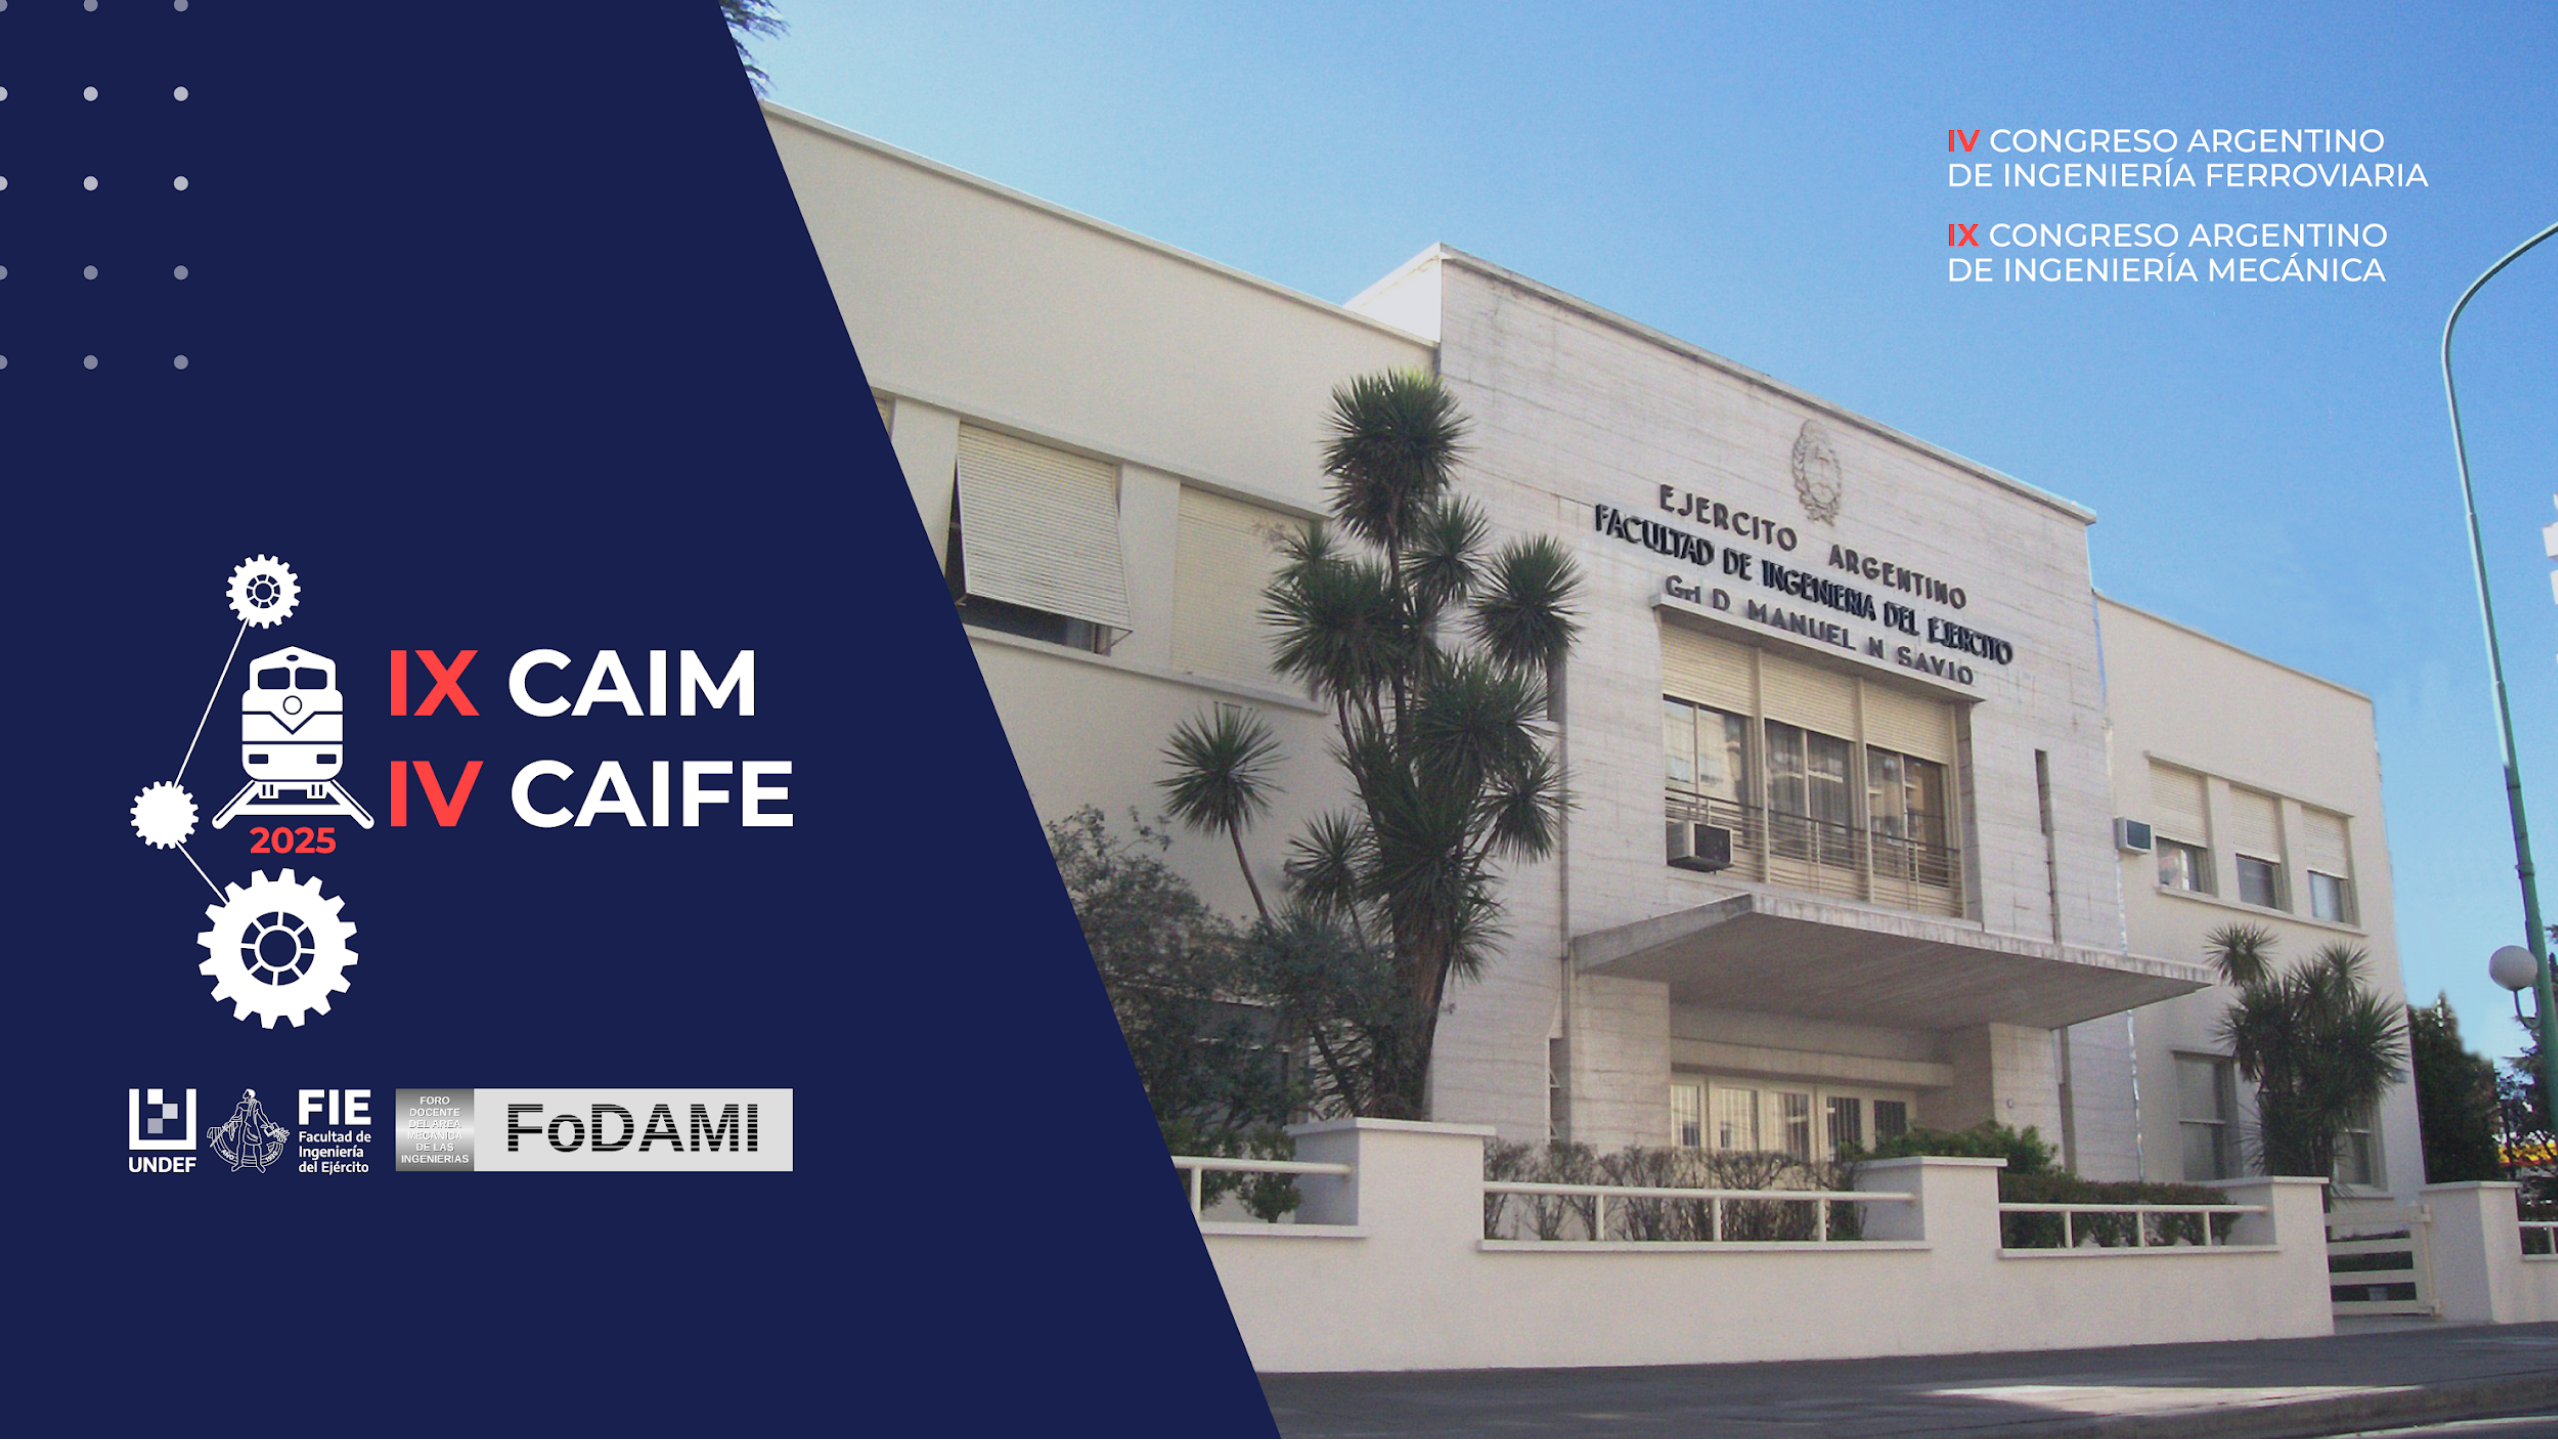
\includegraphics[width=\paperwidth, height=\paperheight]{ersteCAIFE}
} %% https://mprnotes.wordpress.com/2009/08/14/changing-background-image-of-latex-beamer/
\begin{frame}[plain] % plain required for correct page numbering
\end{frame}

\definecolor{caifeblue}{HTML}{18204f}
\setbeamercolor{title}{fg=white,bg=caifeblue}

% Normal blocks
\setbeamercolor{block title}{fg=white,bg=caifeblue}
\setbeamercolor{block body}{fg=black,bg=caifeblue!5!white}



%% Title slide
\usebackgroundtemplate{
  
\includegraphics[width=\paperwidth, height=\paperheight]{titleBackground}
	}	% unset background % https://tex.stackexchange.com/questions/201013/how-to-include-a-background-image-to-only-one-page-of-a-beamer-presentation
\begin{frame}[plain] 
  %\titlepage
 
	\vspace{0.1cm}
	
	\makebox[\textwidth][c]{%
  \begin{beamercolorbox}[wd=0.85\textwidth,sep=4pt,center,rounded=true,shadow=true]{title}
    \usebeamerfont{title}\textbf{Introducción temprana de la mecánica computacional\\
    en cursos de electrostática y mecánica analítica}
  \end{beamercolorbox}%
}
  \vspace{0.1cm}

	\begin{beamercolorbox}[wd=0.21\textwidth,sep=0pt,center,rounded=true,shadow=true]{title}
    \usebeamerfont{title} {\normalsize\textbf{INTEGRANTES }}
  \end{beamercolorbox}
 	
	\vspace{-0.3cm}
 
	\begin{flushleft}
	$\bullet$ Víctor A. Bettachini,
	Dep. de Ingeniería e Investigaciones Técnológicas, UNLaM
	\\
	$\bullet$ Mariano A. Real, Inst. de Calidad Industrial, UNSaM -- INTI
	\\
	$\bullet$ Edgardo Palazzo,
	Dep. de Materias Básicas, UTN--FRA
  \end{flushleft}

  \vspace{0.1cm}

  % Another box
  \begin{beamercolorbox}[wd=0.21\textwidth,sep=0pt,center,rounded=true,shadow=true]{title}
    \usebeamerfont{title} {\normalsize\textbf{SÍNTESIS }}
  \end{beamercolorbox}

	\vspace{-0.3cm}

	\begin{flushleft}
	$\bullet$ Garca
  \end{flushleft}


\end{frame}

% Reset counter after title page
\setcounter{framenumber}{0} % This makes next frame "01"


%% Standard slide
\usebackgroundtemplate{
  
\includegraphics[width=\paperwidth, height=\paperheight]{slideBackground}
} %% https://mprnotes.wordpress.com/2009/08/14/changing-background-image-of-latex-beamer/

\begin{frame}
	\begin{block}{Temario}
		\vspace{0.2cm}
		\tableofcontents
	\end{block}
\end{frame}


\section{Tecnologías en el aula}
\begin{frame}
	\begin{block}{Temario}
		\vspace{0.2cm}
		\tableofcontents[currentsection]
	\end{block}
\end{frame}



\begin{frame}
	\frametitle{Herramientas didácticas}
  %\begin{beamercolorbox}[wd=0.21\textwidth,sep=0pt,center,rounded=true,shadow=true]{frametitle}
  %  \usebeamerfont{title}frametitle
  %\end{beamercolorbox}%
	\begin{columns}
	\begin{column}{0.47 \textwidth}
			\pause
			\begin{block}{Inicio s. XIX: pizarrón y papel}
				\includegraphics[width= \columnwidth]{../figuras/1930s-1940s-man-teacher-professor-vintage-images.jpg}
			\end{block}
		\end{column}
		\pause
		\begin{column}{0.45 \textwidth}
			\begin{block}{Fin s. XX: computadora = ¿proyector?}
				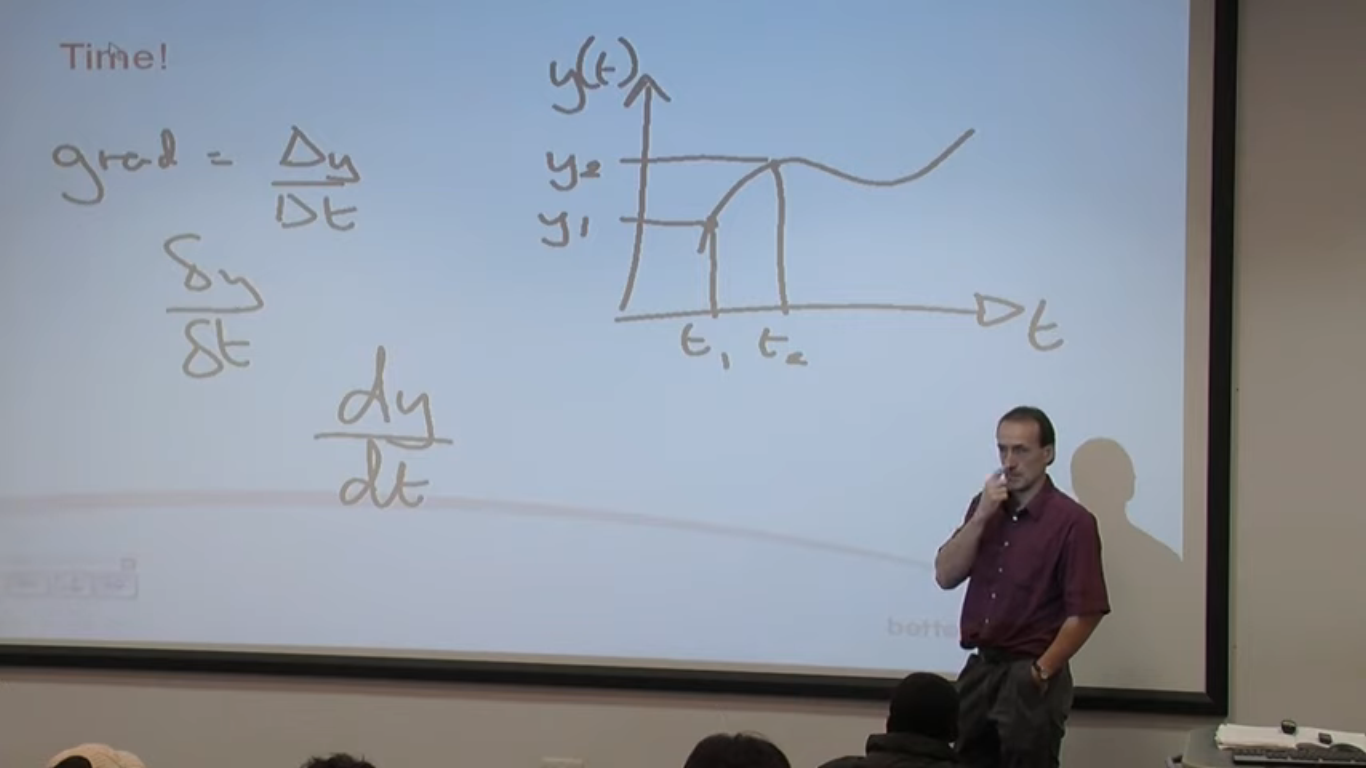
\includegraphics[width= \columnwidth]{../figuras/systemsEngineering.png}
			\end{block}
		\end{column}
	\end{columns}
\end{frame}



\begin{frame}
	\frametitle{Subutilización de la IT}
	\begin{columns}
	\begin{column}{0.47 \textwidth}
			\pause
			\begin{block}{La resistencia al cambio}
				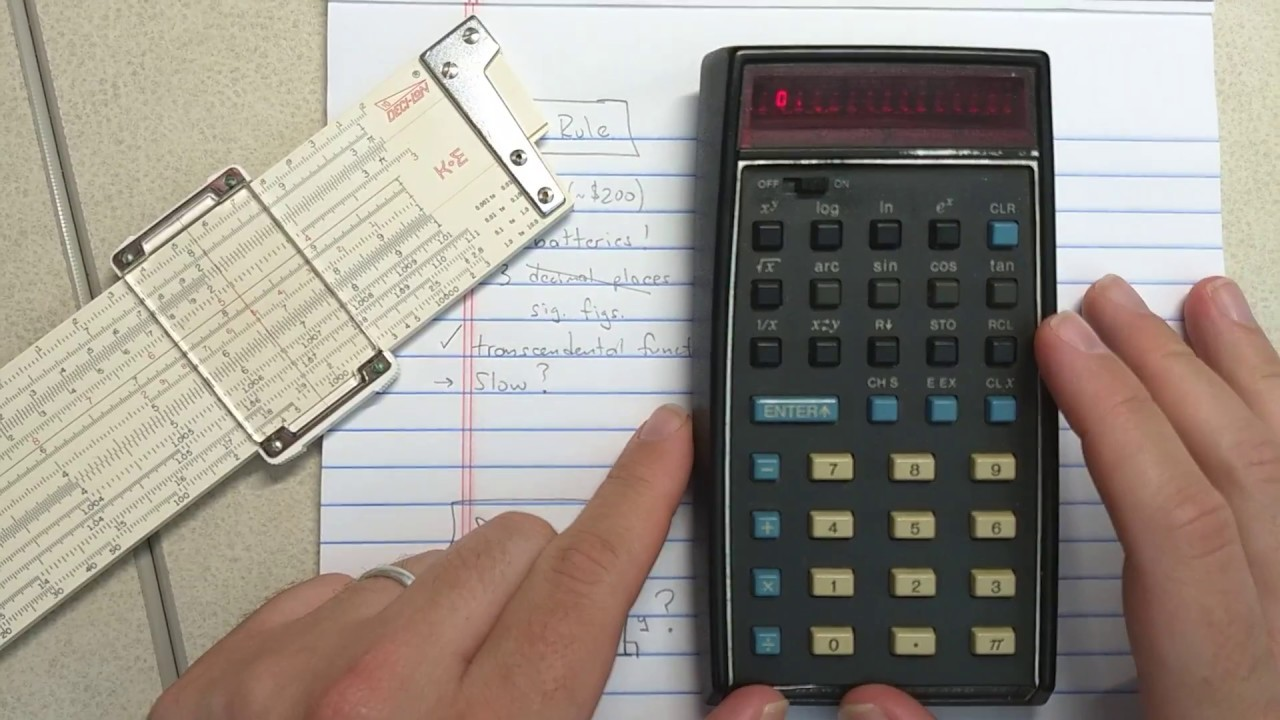
\includegraphics[width= \columnwidth]{../figuras/reglaCalculadora}
			\end{block}
		\end{column}
		\pause
		\begin{column}{0.45 \textwidth}
			\begin{block}{+ 40 años de atraso}
				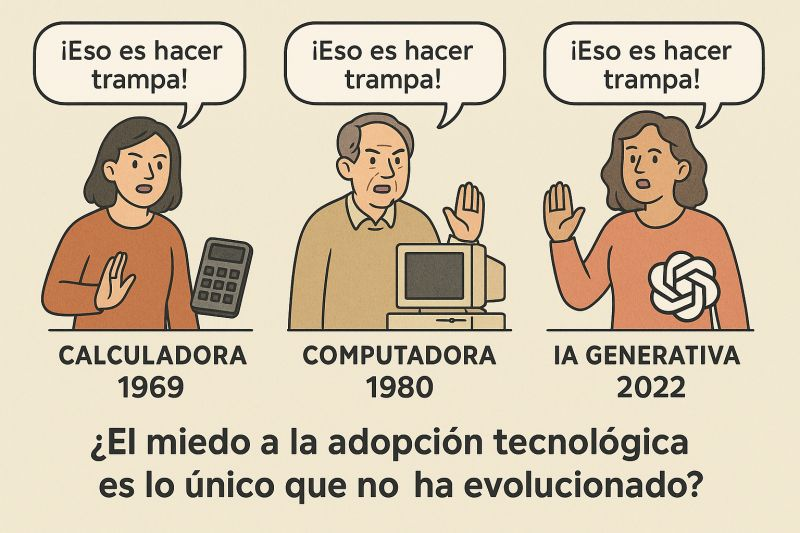
\includegraphics[width= \columnwidth]{../figuras/trap2}
			\end{block}
		\end{column}
	\end{columns}
\end{frame}



\section{¿Código en ingeniería mecánica?}
\begin{frame}
	\begin{block}{}
		\vspace{0.2cm}
		\tableofcontents[currentsection]
	\end{block}
\end{frame}


\begin{frame}
	\frametitle{Mecánica analítica en la UNLaM}
	\begin{columns}
	\begin{column}{0.37 \textwidth}
			\pause
			\begin{block}{Aprobaron álgebras y análisis}
				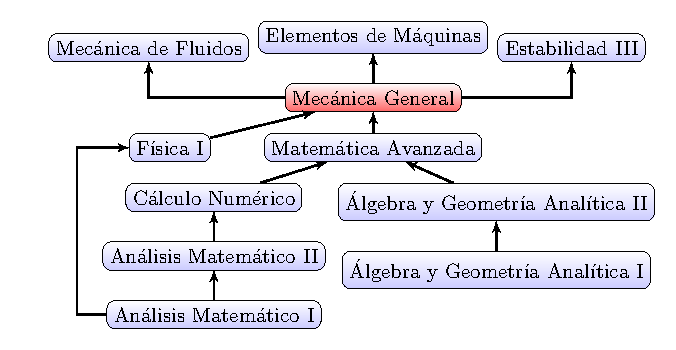
\includegraphics[width= \columnwidth]{../figuras/correlativas_2}
			\end{block}
		\end{column}
		\pause
		\begin{column}{0.55 \textwidth}
			\begin{block}{¿Por qué no automatizarle?}
				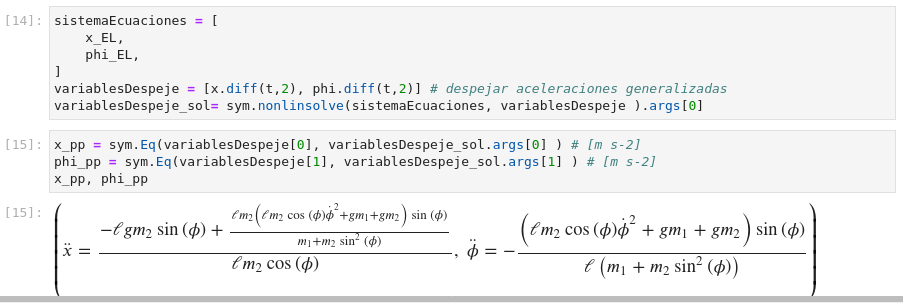
\includegraphics[width= \columnwidth]{../figuras/hard}
			\end{block}
		\end{column}
	\end{columns}
\end{frame}


\begin{frame}
	\frametitle{Valorar el tiempo de docentes y alumnos}
	\pause
	\begin{block}{}
	  \begin{columns}[b]
			\begin{column}{0.25\textwidth}
				\includegraphics[width= \columnwidth]{1930s-1940s-man-teacher-professor-vintage-images}
			\end{column}
			\begin{column}{0.65\textwidth}
				\begin{itemize}[<+->]
					\item Profesor: prepara lecciones \(\xrightarrow{de\, memoria}\) pizarrón/presentación
					\item Estudiante: del pizarrón/presentación \(\xrightarrow{transcribe}\) propio cuaderno
					\item Práctica: \textbf{rehacer} los mismo cálculos, diagramas, etc\dots
					\item Aburrimiento \(\implies \downarrow\) pérdida de concentración en la clase
				\end{itemize}
			\end{column}
		\end{columns}
	\end{block}
	\pause
	Licklider (1957): 85\% de ``pensar'' es lo mundano (calcular, dibujar, etc.)
	\pause
	\begin{block}{}
	  \begin{columns}[b]
			\begin{column}{0.3\textwidth}
				\includegraphics[width= \columnwidth]{"Screenshot 2023-09-18 at 12-24-03 Google Colaboratory"}
			\end{column}
			\begin{column}{0.65\textwidth}
				\begin{itemize}[<+->]
					\item Profesor: ideas \(\xrightarrow{actualiza}\) código/teoría en repositorio
					\item Estudiante: repositorio del curso \(\xrightarrow{Correlacionar}\) propio repositorio
					\item \textbf{Recicla} código del profesor para resolver nuevos problemas
				\end{itemize}
			\end{column}
		\end{columns}
	\end{block}
\end{frame}



\section{Herramientas de este siglo para el aula}
\begin{frame}
	\begin{block}{Temario}
		\vspace{0.2cm}
		\tableofcontents[currentsection]
	\end{block}
\end{frame}


\begin{frame}
	\frametitle{Cuaderno Jupyter: texto + ecuaciones + código ejecutable}
	%\pause
	\begin{block}{}
	% \begin{block}{On-line programmable notebook: text + equations + code}
		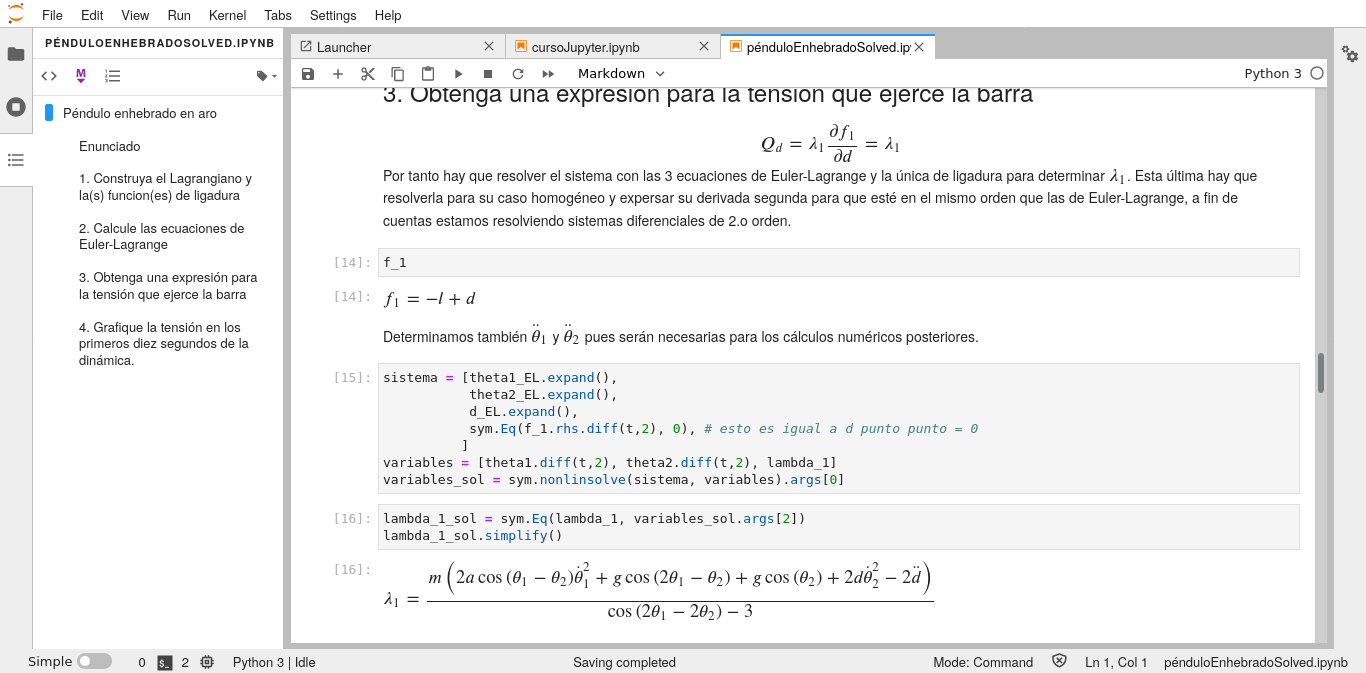
\includegraphics[width= \columnwidth]{screenshot_JupyterLab}
	\end{block}
\end{frame}


\begin{frame}
\frametitle{Google Colaboratory: cuadernos Jupyter en la nube}
	% \pause
	\begin{block}{}
		% \begin{itemize}[<+->]
		\begin{itemize}
			\item Profesor puede editar y comentar el trabajo del alumno.
			% \item It runs Jupyter notebooks online, and it's free.
			\item Múltiples estudiantes pueden trabajar el mismo cuaderno en forma remota.
		\end{itemize}
		% \uncover<4->{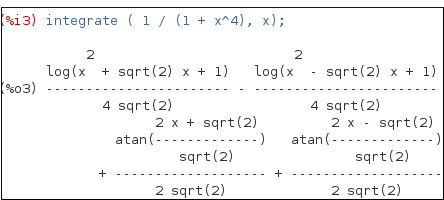
\includegraphics[height= 2cm]{ucarecdn}}
		\begin{center}
			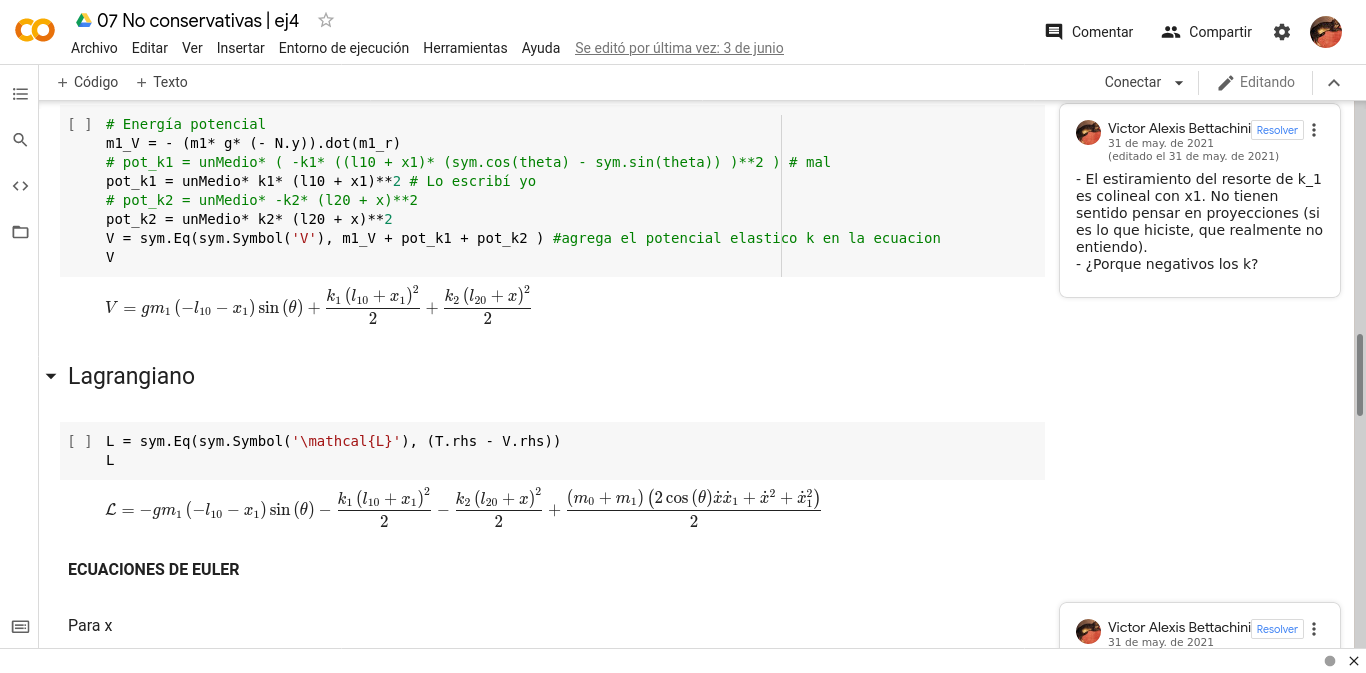
\includegraphics[width= 0.8\textwidth]{comentariosColab}
		\end{center}
	\end{block}
	% \pause
\end{frame}


\begin{frame}
	\frametitle{Repositorio GitHub}
	% \pause 
	\begin{block}{}
		% \begin{itemize}[<+->]
		\begin{itemize}
			\item Organizado por tema, acceso libre, fácil de actualizar.
			\item Google Colaboratory carga cuadernos Jupyter  directamente desde GitHub.
		\end{itemize}
		% \uncover<4->{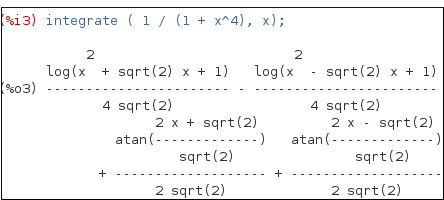
\includegraphics[height= 2cm]{ucarecdn}}
		\begin{center}
			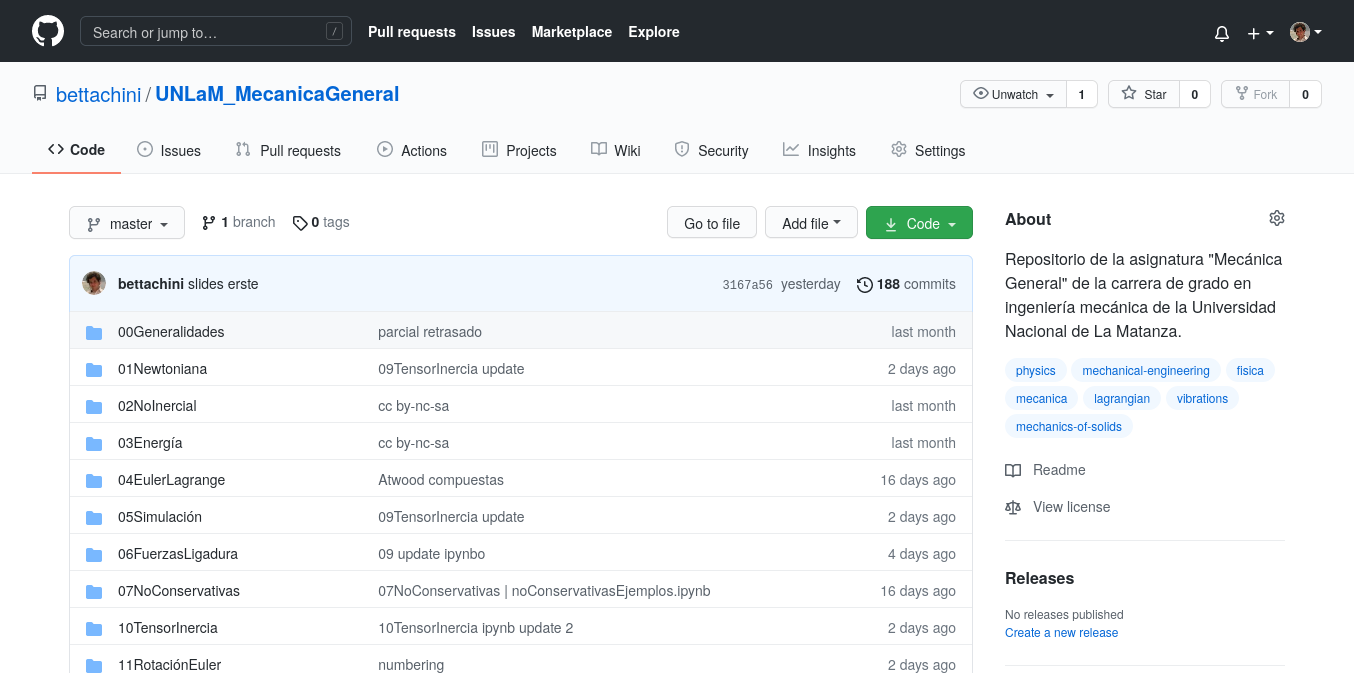
\includegraphics[width= 0.8\textwidth]{repositorioGithub}
		\end{center}
	\end{block}
	% \pause
\end{frame}


\begin{frame}
	\frametitle{\LaTeX \,: notación matemática concisa}
	% \pause
	\begin{block}{}
		\begin{itemize}
			\item \LaTeX \, sigue el estandar de la American Mathematical Society
		\end{itemize}
		% \uncover<4->{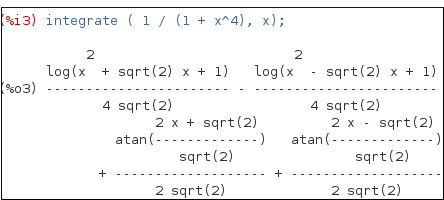
\includegraphics[height= 2cm]{ucarecdn}}
		\begin{center}
			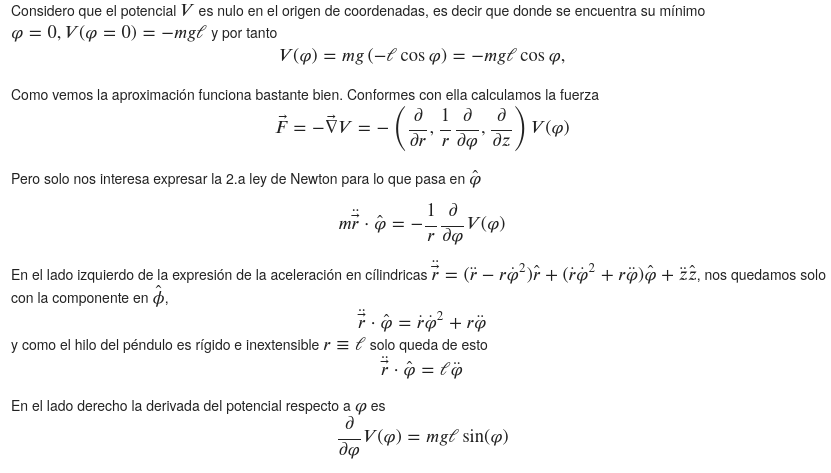
\includegraphics[width= 0.8\textwidth]{clase1péndulo}
		\end{center}
	\end{block}
	% \pause
\end{frame}


%\begin{frame}
%	\frametitle{1er clase | Matplotlib: precise and reproducible graphics}
%	% \pause
%	\begin{block}{}
%		\begin{itemize}
%			\item Explicit Python code for producing graphics. Students are enticed to play with it.
%		\end{itemize}
%		% \uncover<4->{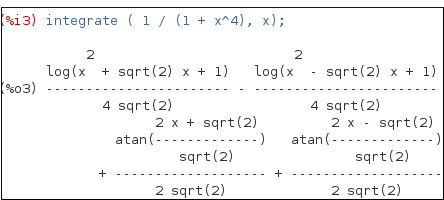
\includegraphics[height= 2cm]{ucarecdn}}
%	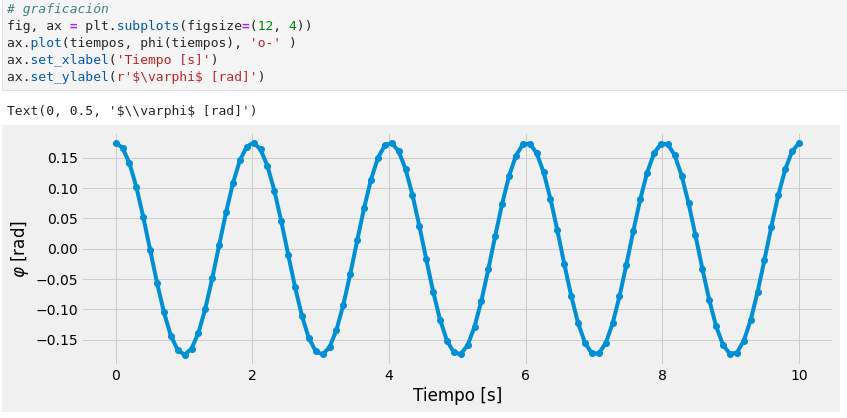
\includegraphics[width= 0.8\textwidth]{clase1gráficos}
%	\end{block}
%	% \pause
%\end{frame}


\begin{frame}
	\frametitle{1er clase | SymPy: álgebra y análisis simbólico}
	% \pause
	\begin{block}{}
		\begin{itemize}
			\item El esfuerzo del estudiante se centra en la nueva temática
		\end{itemize}
		% \uncover<4->{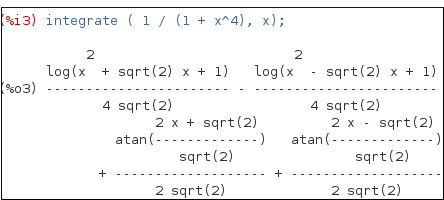
\includegraphics[height= 2cm]{ucarecdn}}
		\begin{center}
			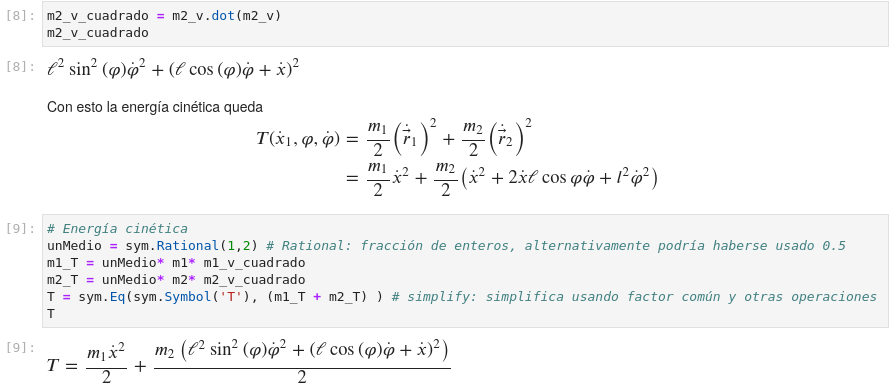
\includegraphics[width= 0.9\textwidth]{clase3sympy}
		\end{center}
	\end{block}
	% \pause
\end{frame}


\begin{frame}
	\frametitle{3er clase | Dinámica por Euler-Lagrange}
	% \pause
	\begin{block}{}
		% \uncover<4->{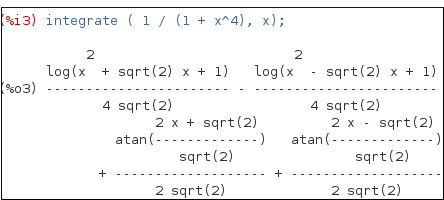
\includegraphics[height= 2cm]{ucarecdn}}
		\begin{center}
			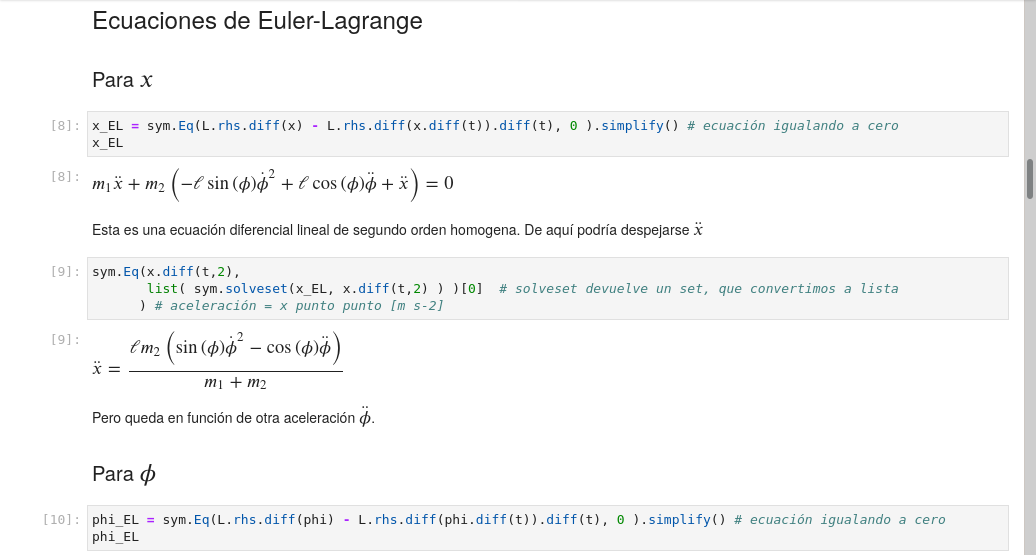
\includegraphics[width= 0.9\textwidth]{clase5EulerLagrange.png}
		\end{center}
	\end{block}
	% \pause
\end{frame}


%\begin{frame}
%	\frametitle{Tools | 4th class | Automatation of resolutions}
%	% \pause
%	\begin{block}{}
%		\begin{itemize}
%			% \item No heavy calculations consuming the energy of the students.
%			\item Mathematical complexity doesn't limit the scope of tackled mechanical problems.
%		\end{itemize}
%		% \uncover<4->{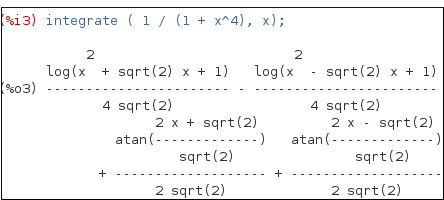
\includegraphics[height= 2cm]{ucarecdn}}
%	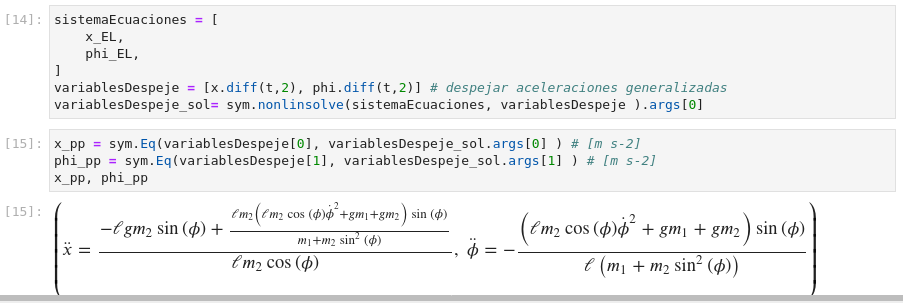
\includegraphics[width= \textwidth]{clase4Aceleraciones}
%	\end{block}
%	% \pause
%\end{frame}


\begin{frame}
	\frametitle{5ta clase | SciPy: cálculo numérico}
	% \pause
	\begin{block}{}
		%\begin{itemize}
		%	\item Explicit solutions.
		%\end{itemize}
		% \uncover<4->{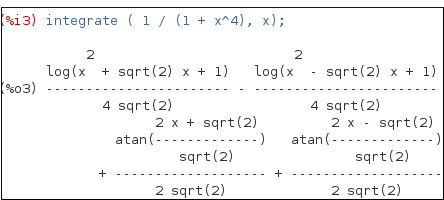
\includegraphics[height= 2cm]{ucarecdn}}
		\begin{center}
			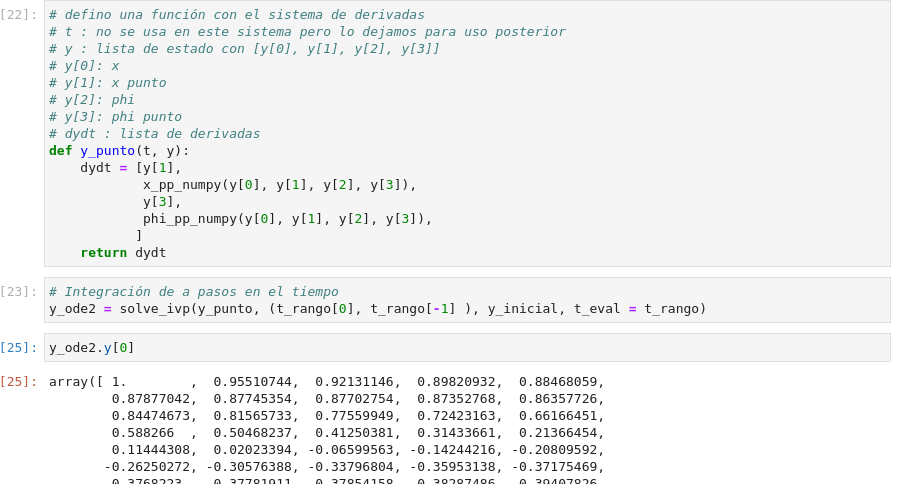
\includegraphics[width= 0.9\textwidth]{clase5Soluciones.png}
		\end{center}
	\end{block}
	% \pause
\end{frame}


\begin{frame}
	\frametitle{5ta clase | Análisis gráfico de resultados}
	% \pause
	%Class 5: analysis of results
	\begin{block}{}
		% \uncover<4->{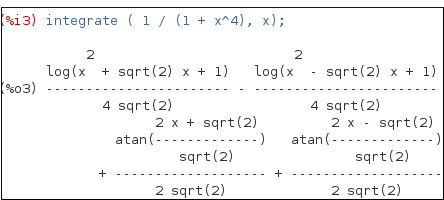
\includegraphics[height= 2cm]{ucarecdn}}
		\begin{center}
			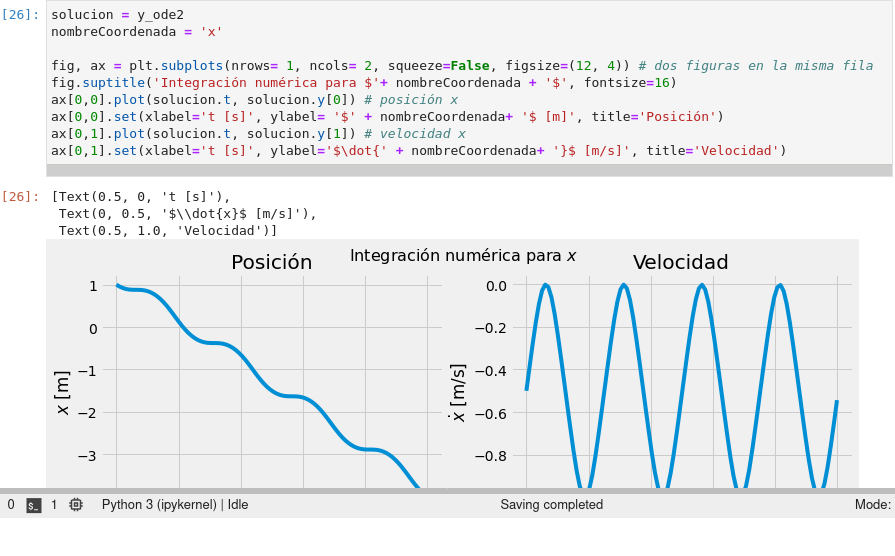
\includegraphics[width= 0.9\textwidth]{clase5Representación}
		\end{center}
	\end{block}
	% \pause
\end{frame}



\begin{frame}
	\frametitle{7ma clase | Fuerzas no conservativas y de ligadura}
	% \pause
	%Class 7: Adding complexity
	%\begin{minipage}{0.6\linewidth}
	\begin{block}{}
%		\begin{itemize}
%			\item Code from previous classes is \textbf{recycled} to model more realistic devices.
%			%\item Gradual increase in complexity of simulated mechanical devices.
%		\end{itemize}
		% \uncover<4->{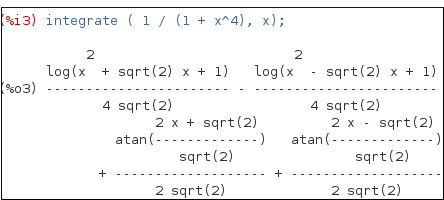
\includegraphics[height= 2cm]{ucarecdn}}
		\begin{center}
			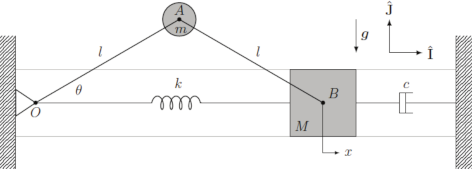
\includegraphics[width= 0.4\columnwidth]{clase7esquema.png}\\
			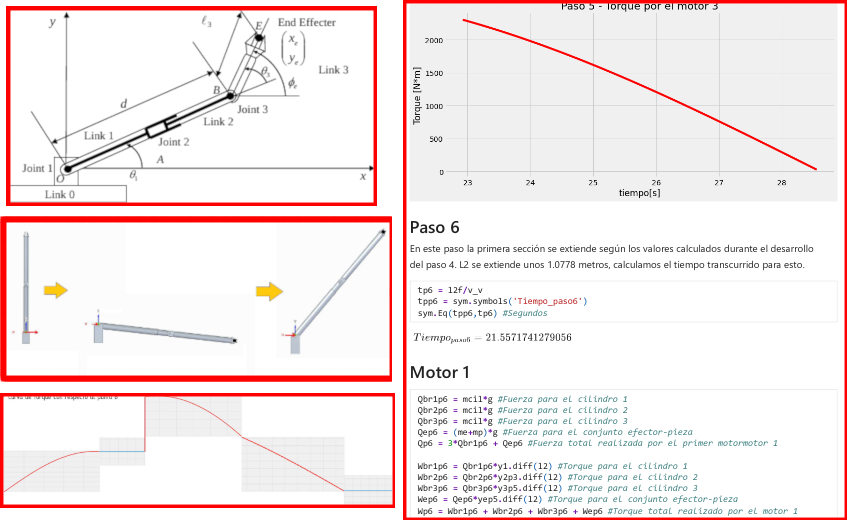
\includegraphics[width= 0.6\columnwidth]{robotArm.png}
		\end{center}
%	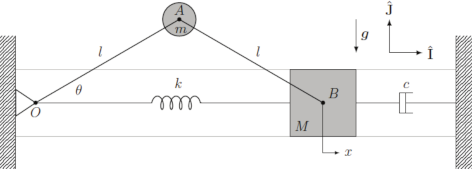
\includegraphics[height= 3.35 cm]{clase7esquema.png}
%	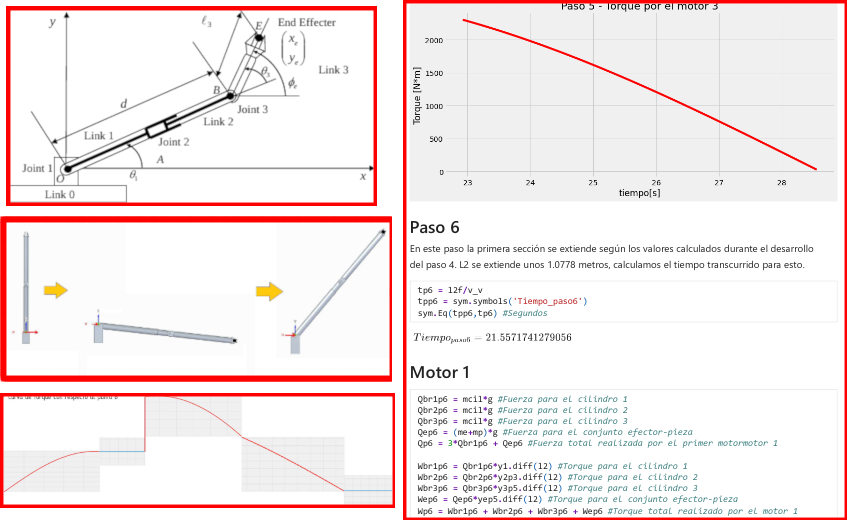
\includegraphics[height= 3.35 cm]{robotArm.png}
	\end{block}
	%\end{minipage}
	% \pause
\end{frame}


\begin{frame}
	\frametitle{8va clase | GitHub Copilot: código de un LLM}
	% \pause
	%Class 7: Adding complexity
	\begin{block}{}
		\begin{itemize}
			\item Tras dominar lo básico los estudiantes pueden aprovecharse de la IA.
			%\item Gradual increase in complexity of simulated mechanical devices.
		\end{itemize}
		% \uncover<4->{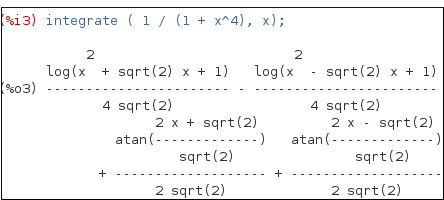
\includegraphics[height= 2cm]{ucarecdn}}
		\begin{center}
			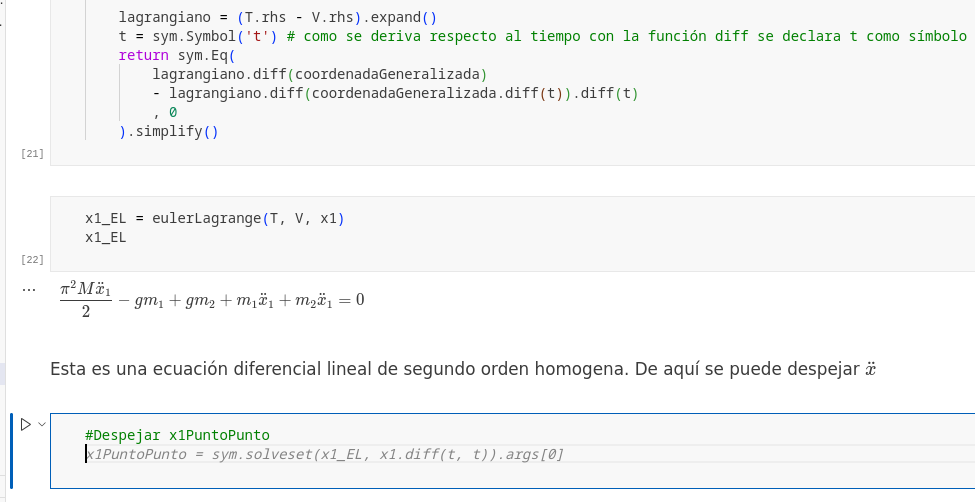
\includegraphics[width= 0.85\textwidth]{copilot}
		\end{center}
	\end{block}
	% \pause
\end{frame}



\begin{frame}
	\frametitle{Clase invertida | Ciclo semanal}
	\begin{block}{}
	% \begin{block}{New theory alongisde its worked examples in programmable notebooks}
		\begin{itemize}[<+->]
			\item Cuadernos Jupyter con la nueva teoría y guías de ejercicios publicadas en línea.
			\item Ejercicios de la semana anterior \textbf{deben} entregarse para evaluación.
			\item Consultas \textbf{asincrónicas} en línea 24/7 son \textbf{públicas} para otros estudiantes.
			\item Encuentros \textbf{sincrónicos} con auxiliares para finalizar ejercicios.
%			%\item \textbf{Remote collaboration} on multi-user notebooks
			%\item Weekly meetings to \textbf{synchronically} unfinished assignments with TA's assistance
			% \item On a weekly basis these \textbf{must} be turned-in for scoring
		\end{itemize}
	\end{block}
	\begin{columns}[b]<1->
    \begin{column}{0.4\textwidth}
			\begin{block}{}
			%\begin{block}{Flipped classroom}
				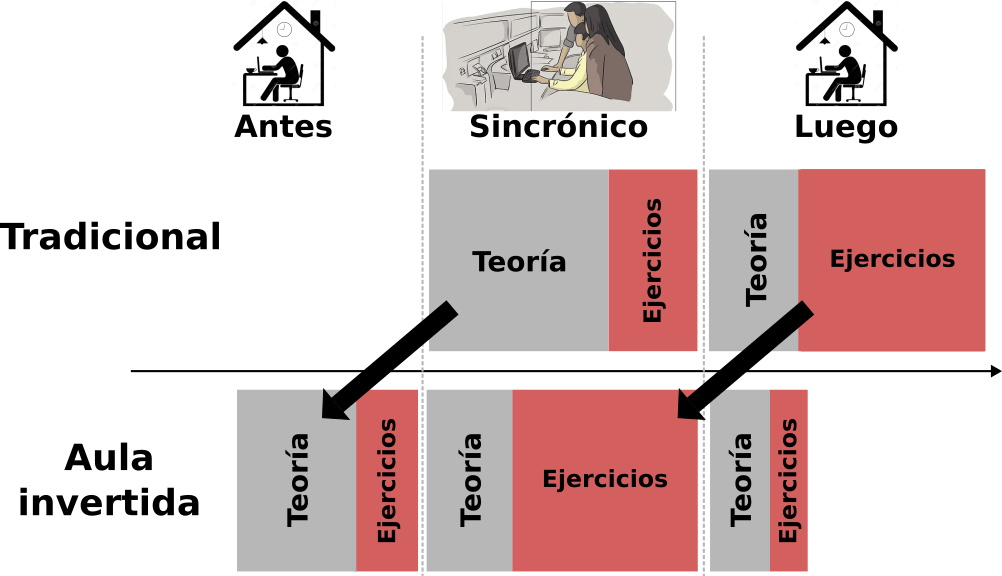
\includegraphics[width= \columnwidth]{flippedClassroomSchedule_castellano.png}
			\end{block}
    \end{column}
    \begin{column}{0.55\textwidth}
			\begin{block}{}
				\begin{tabular}{lll}
					\hline
					Sincrónico & Teoría & Ejercicios\\
					\hline
					Antes & Leer y aplicar & Iniciarles\\
					Durante & Consultas & Completarles\\
					% Durante & Aclarar dudas & \begin{tabular}{@{}c@{}}Terminarles\\(semanal)\end{tabular}\\
					Luego & \begin{tabular}{@{}l@{}}Aclaraciones\\adicionales\end{tabular} & \begin{tabular}{@{}l@{}}Ayuda de auxiliares\end{tabular}\\
					\hline
				\end{tabular}
			\end{block}
    \end{column}
  \end{columns}
\end{frame}


%\begin{frame}
%	\frametitle{Methodology | Google Colaboratory: asynchronic remote assistance}
%	\begin{block}{}
%	% \begin{block}{Student's work can be commented and edited in Google Colaboratory}
%		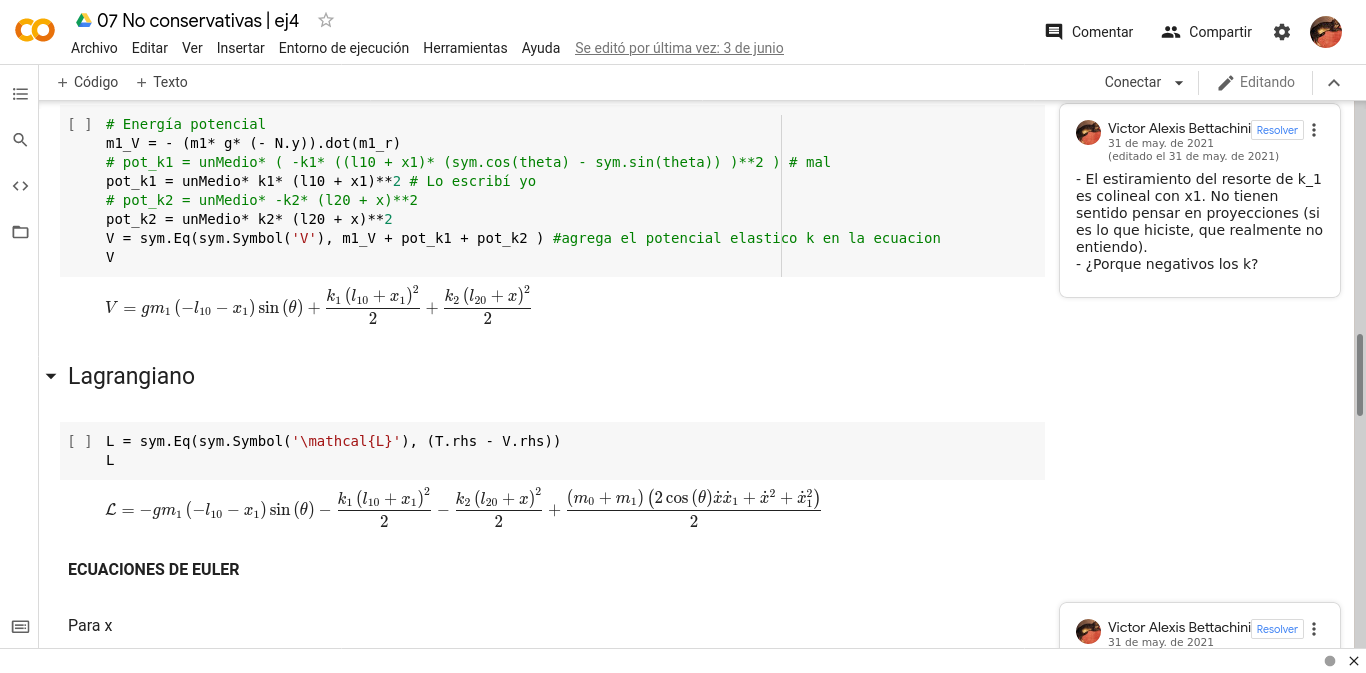
\includegraphics[width= \columnwidth]{comentariosColab}
%	\end{block}
%\end{frame}



\begin{frame}
	\frametitle{Microsoft Teams: seguimiento individualizado}
	\begin{block}{Registro semalas de entregas de ejercicios}
		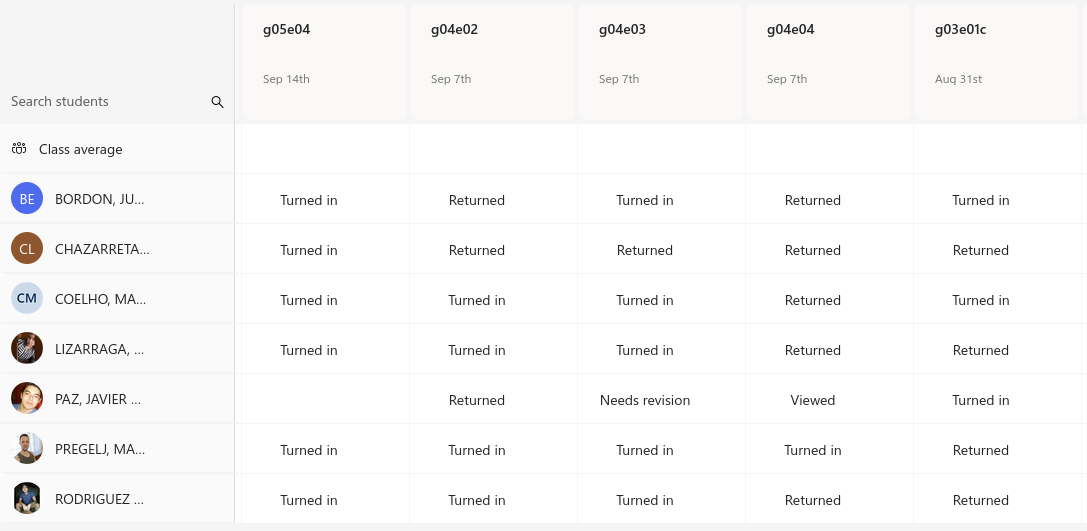
\includegraphics[width= 0.9\columnwidth]{seguimiento}
	\end{block}
\end{frame}


%\begin{frame}
%	\frametitle{Methodology | Exams are just another assignment}
%	\begin{block}{}
%	% \begin{block}{The exam is just another excercise.}
%		\begin{itemize}
%			\item The students send their notebook file.
%			\item Feedback is inserted in between the student's work.
%		\end{itemize}
%		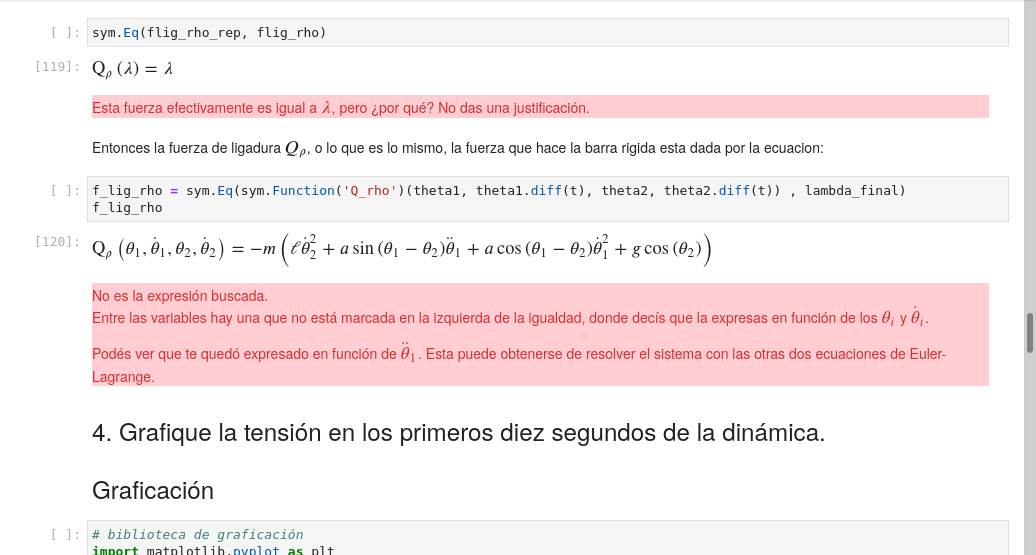
\includegraphics[width= \columnwidth]{parcial}
%	\end{block}
%\end{frame}



\begin{frame}
	\frametitle{UNLaM | Difusión de la IT}
	Repo GitHub

	Captura de publicación en JOSE
\end{frame}




\begin{frame}
	\frametitle{UNLaM | Mecánica Analítica}
	\begin{columns}[c]
    \begin{column}{0.44 \textwidth}
			\begin{block}{Repositorio GitHub}
				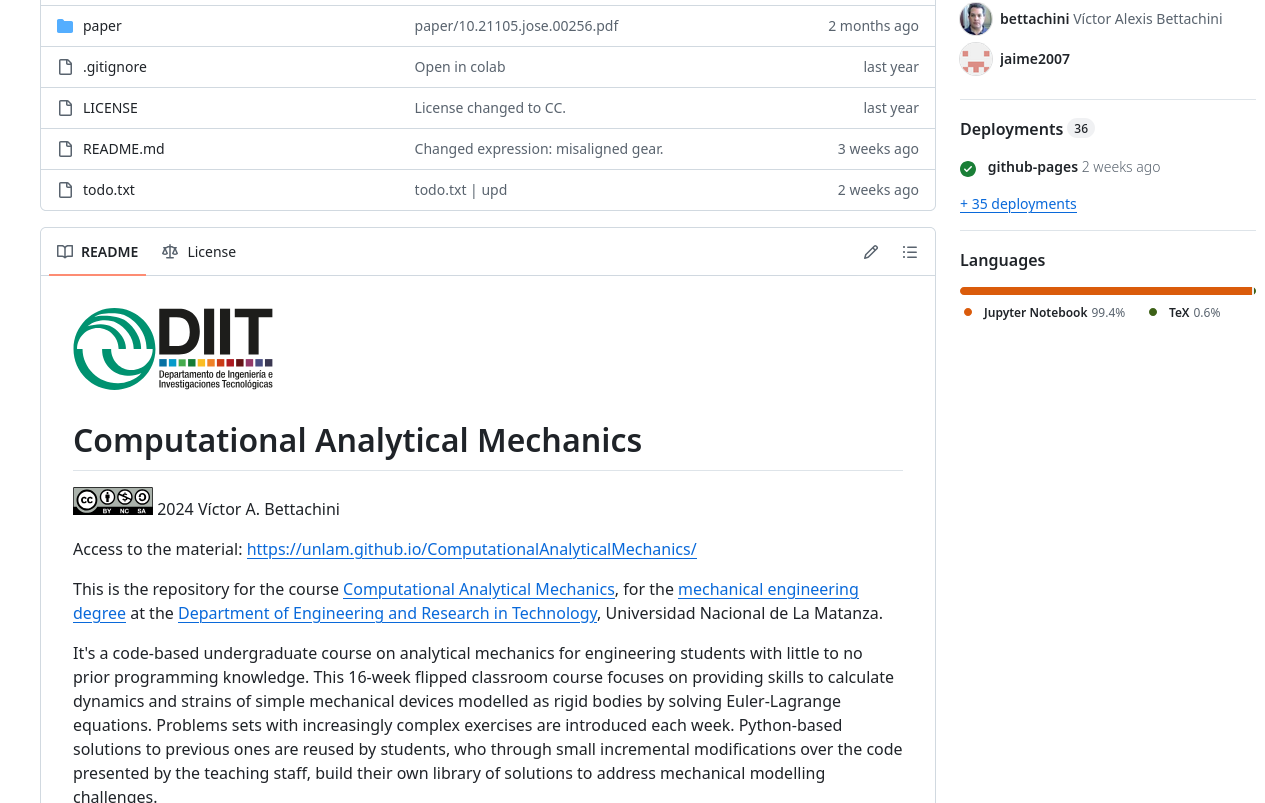
\includegraphics[width= \columnwidth]{gitHubCAM}
			\end{block}
    \end{column}
		\begin{column}{0.5 \textwidth}
			\begin{block}{Journal Open Source Education}
				
\includegraphics[width= \columnwidth]{joseCAM}
			\end{block}
		\end{column}
		\end{columns}
\end{frame}




%\begin{frame}
%	\frametitle{UNLaM | Aula invertida}
%	\begin{columns}[c]
%    \begin{column}{0.6 \textwidth}
%			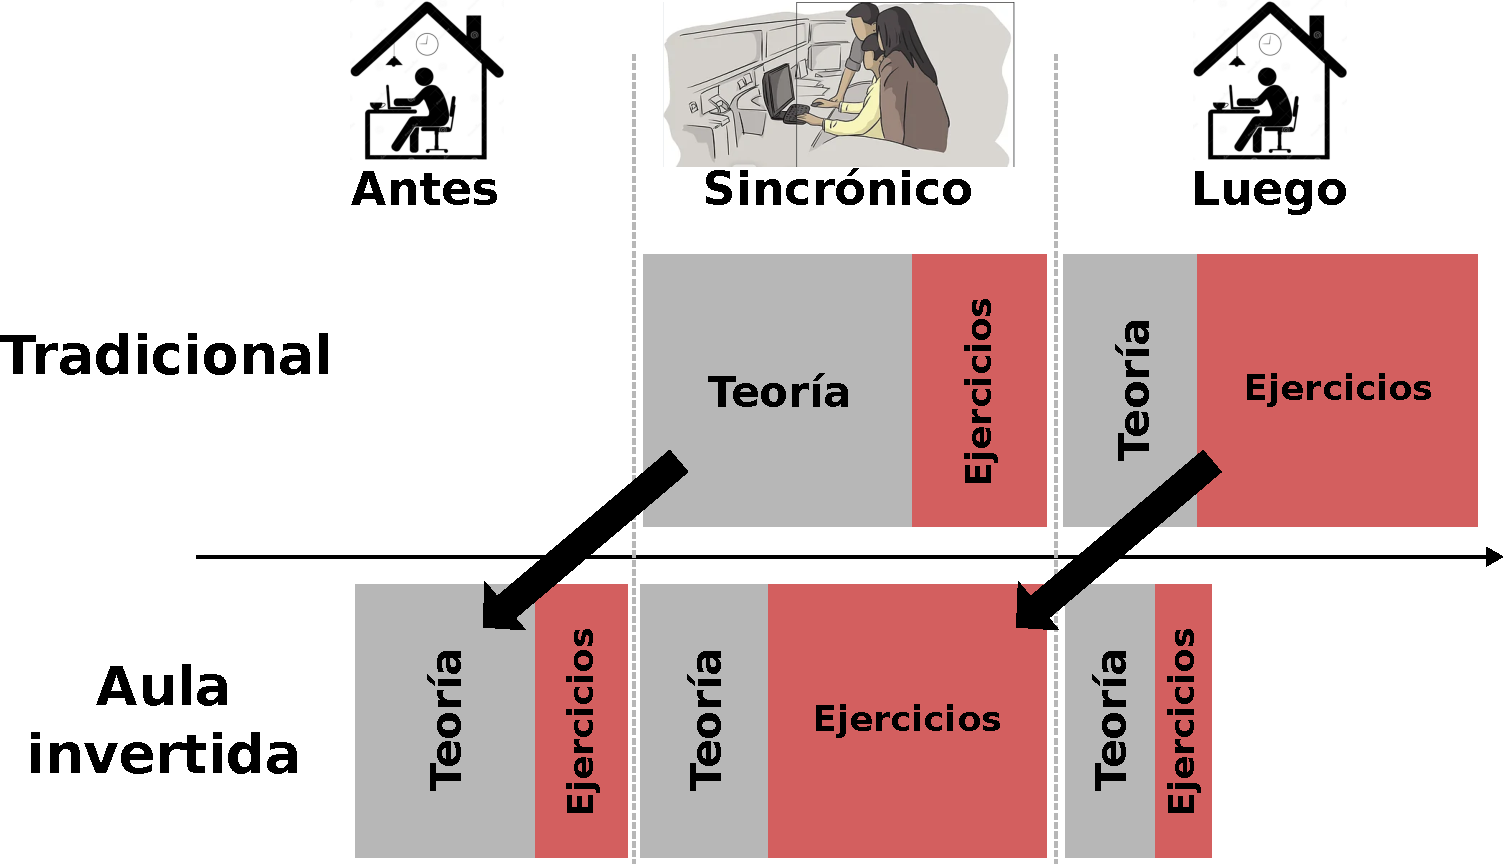
\includegraphics[width= \columnwidth]{aulaInvertidaHorario}
%    \end{column}
%		\begin{column}{0.4 \textwidth}
%			\pause
%			La encuesta y gráficos de sus resultados
%      \begin{itemize}[<+->]
%      % \begin{enumerate}[<+->]
%         \item Campos magnéticos
%         \item Campos eléctricos
%         \item Temperatura
%				 \item Vibraciones
%				 \item Presión atmosférica
%      \end{itemize}
%      % \end{enumerate}
%    \end{column}
%  \end{columns}
%\
%\end{frame}




\section{UNLaM | Física III}

\begin{frame}
	\frametitle{UNLaM | Física III}
	Contar del curso y de los ejercicios hechos en Google Colab.
\end{frame}


\begin{frame}
	\frametitle{UNLaM | Resultados en curso Física III }
 \begin{columns}[c]
    \begin{column}{0.6 \textwidth}
			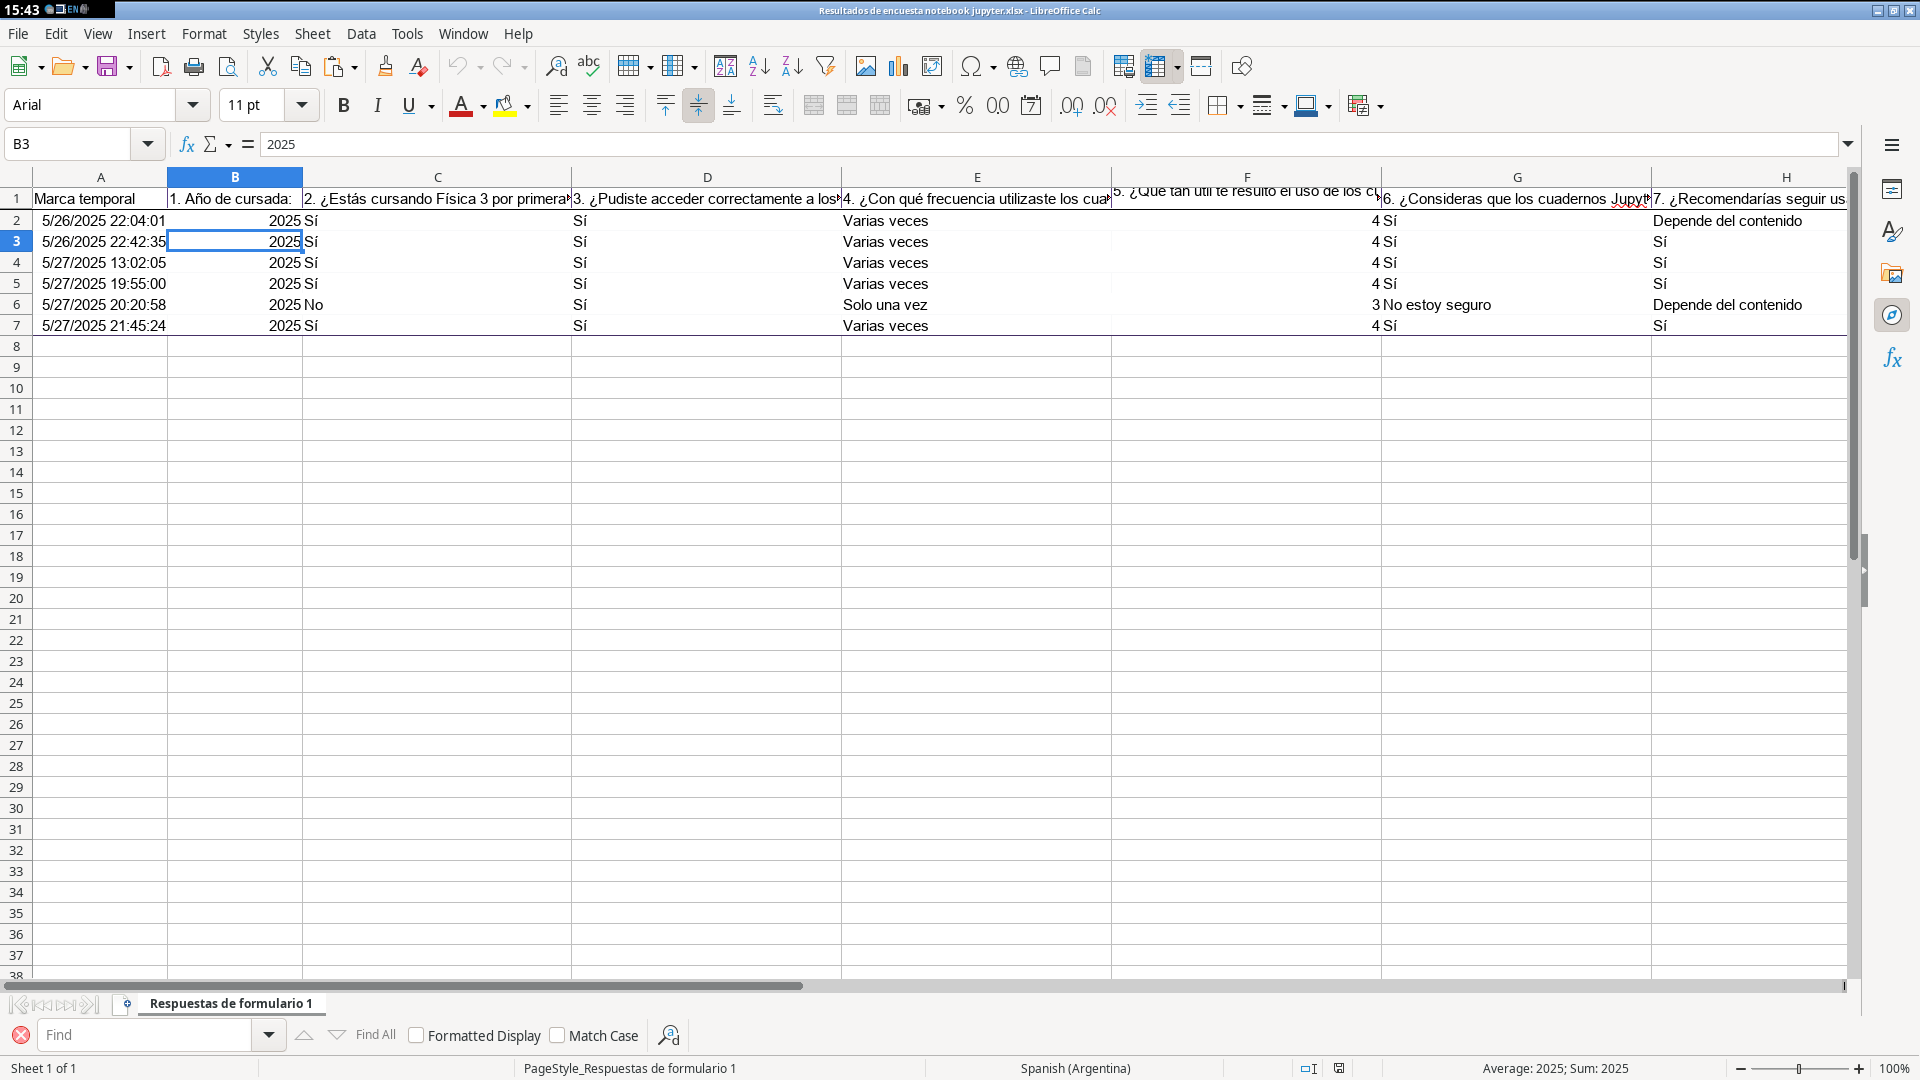
\includegraphics[width= \columnwidth]{2025-07-18-154309_1920x1080_scrot.png}
    \end{column}
		\begin{column}{0.4 \textwidth}
			\pause
			La encuesta y gráficos de sus resultados
      \begin{itemize}[<+->]
      % \begin{enumerate}[<+->]
         \item Campos magnéticos
         \item Campos eléctricos
         \item Temperatura
				 \item Vibraciones
				 \item Presión atmosférica
      \end{itemize}
      % \end{enumerate}
    \end{column}
  \end{columns}
\end{frame}



\section{UTN | Física II}

\begin{frame}
	\frametitle{UTN | Física II}
	Electrostática \& co.
\end{frame}


\section{UTN | Física II}
\begin{frame}
	\frametitle{UTN | Resultados en Física II}
	Resultados sin herramientas de cálculo
\end{frame}



\begin{frame}
	\frametitle{Etapas hacia una implementación}
	\begin{enumerate}[<+->]
		\item Contar con muchos ejemplos de anomalías
		\begin{itemize}
			\item Series provistas por Gertsvolf del National Research Council de Canadá
		\end{itemize}
		\item Implementación local de algoritmos Sub-LOF y CPD
		\begin{itemize}
			\item Reproducir resultados de Chen et al. (2024) con series provistas
		\end{itemize}
		\item Minar series de tiempo propias en búsqueda de anomalías
		\begin{itemize}
			\item Evaluar número de anomalías detectadas con Sub-LOF y CPD
		\end{itemize}
		\item Correlacionar anomalías en tiempo con las de parámetros
		\begin{itemize}
			\item Registrar series temporales de parámetros internos y ambientales
			\item Detección \emph{clásica} (Z-score, ARIMA) o con ML (autoencoder)
			\item Evaluar algoritmos de correlación temporal de sucesos entre series
		\end{itemize}
	\end{enumerate}
\end{frame}


% Closing slide
\usebackgroundtemplate{
  
\includegraphics[width=\paperwidth, height=\paperheight]{lastCAIFE}
} %% https://mprnotes.wordpress.com/2009/08/14/changing-background-image-of-latex-beamer/
\begin{frame}[plain] % plain required for correct page numbering
\end{frame}



\end{document}
